\documentclass[pdftex,12pt,a4paper]{article}
%\documentclass{report}
\usepackage{amsmath}
\usepackage{amssymb}
\usepackage{fullpage}
\usepackage{pdfpages}
\usepackage{listings}
\usepackage{longtable}
\usepackage{verbatim}
\usepackage{algorithm}
\usepackage{algpseudocode}
\usepackage{url}
\usepackage{listings}
\newcommand{\HRule}{\rule{\linewidth}{0.5mm}}
\newcommand{\nspace}{\\[0.25cm]}
\newcommand{\lspace}{\\[0.50cm]}
\newcommand{\Lspace}{\\[1.0cm]}
\newcommand{\LSPACE}{\\[2.0cm]}


\title{Design and Analysis of Algorithms Course Project}
\author{Jonathan Gillett \& Joseph Heron \& Amit Jain}



\begin{document}
\pagestyle{empty}
\begin{titlepage}
  		\newlength{\saveparindent}
		\setlength{\saveparindent}{\parindent}
		\setlength{\parindent}{0cm}
  		\sf
		\center
 
  		\HRule\\[0.60cm]
			\textsc{\Huge Design and Analysis of Algorithms}\\[0.25cm] 
			\textsc{\Huge Course Project}\\[0.50cm]
		\HRule\\[6.5cm]
		\textsc{\LARGE Jonathan Gillett \qquad Joseph Heron}\\[0.65cm]
		\textsc{\LARGE Amit Jain}\\[6.5cm]
		\textsc{\LARGE{}\today}\\

  		\setlength{\parindent}{\saveparindent}
\end{titlepage}


% Flush everything to the left
\flushleft


\textsc{\Huge Convex Hull Algorithm} \hfill \Lspace


% Description of convex hull algorithms (take from wikipedia
\textsc{\Large Description} \hfill \nspace

The convex hull is the set of points such that they form the smallest convex hull that encompasses the set of all points within the hull. A typical analogy for the convex hull is that it can be thought of as a set of points, such that when a rubber band is stretched around them it forms the
convex hull of a set of points.

\begin{figure}[h!]
  \centering
	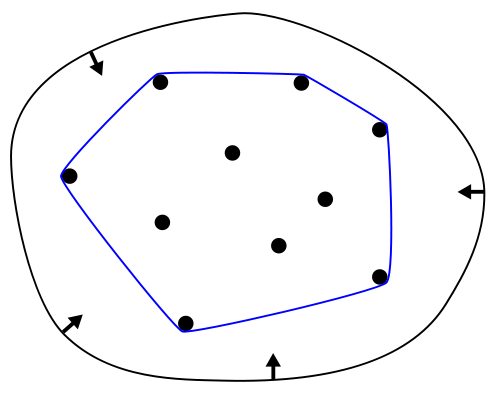
\includegraphics[scale=0.4]{img/convexhull_rubberband.png}
	\caption{http://commons.wikimedia.org/wiki/Image:ConvexHull.png}
\end{figure}

The convex hull algorithms are used to determine the convex hull of a finite set of points,
currently there are several well-known algorithms used to determine the convex hull of a finite
set of points such as: Jarvis March, Graham Scan, QuickHull, Monotone Chain, Marriage-Before-Conquest, and Chan's Algorithm.  Currently the best algorithmic complexity for the convex hull algorithm is $O(n log h)$, which Chan's algorithm being the most recently published optimal  convex hull algorithm.\cite{chan1996optimal}\nspace

% ADD CITATION FOR BIG-O COMPLEXITY

For our project we decided to use the Monotone Chain algorithm, which has a worst-case complexity
of $O(n log n)$, while it is not as optimal as Chan's algorithm or Marriage-Before-Conquest the Monotone Chain algorithm is better understood and more widely used due to the ease of impementation.\Lspace

% Citation



% Description of algorithm, explanation of the code
\textsc{\Large Monotone Chain Algorithm} \hfill \nspace

For the Monotone Chain algorithm the upper and lower hulls will then be constructed through the use of cross product. The cross product is used to check if adding the point to the hull will case it to have a counter-clockwise turn. In other words, the addition of the point would cause the polygon to no longer be a convex hull since it would contain a concave section.\nspace

The Monotone Chain algorithm starts by first sorting the points lexicographically and then constructs the upper and lower hulls of the points using the cross product to check if adding the points to the hull will cause it to have a counter-clockwise turn. In our implementation we use the QuickSort algorithm to first sort the points and then we use the cross product when constructing the upper and lower hull.\nspace

As part of our research into the Monotone Chain algorithm we first did research into the
pseudocode for the algorithm, eventually we came across an excellent web article by Dan Sunday,
which provided detailed pseudocode and explanations of the Monotone Chain Algorithm.\cite{website:monotonechainweb} The following pseudocode for the Monotone Chain Algorithm was used to aid in our own implementation of the algorithm in Python.

\begin{verbatim}

Input: a set S = {P = (P.x,P.y)} of N points

    Sort S by increasing x- and then y-coordinate.
    Let P[] be the sorted array of N points.

    Get the points with 1st x min or max and 2nd y min or max
      minmin = index of P with min x first and min y second
      minmax = index of P with min x first and max y second
      maxmin = index of P with max x first and min y second
      maxmax = index of P with max x first and max y second

    Compute the lower hull stack as follows:
    (1) Let L_min be the lower line joining P[minmin] with P[maxmin].
    (2) Push P[minmin] onto the stack.
    (3) for i = minmax+1 to maxmin-1  (between the min and max)
        {
            if (P[i] is above or on L_min)
                Ignore it and continue.
            while (there are at least 2 points on the stack)
            {
                Let PT1 = the top point on the stack.
                Let PT2 = the second point on the stack.
                if (P[i] is strictly left of the line from PT2 to PT1)
                    break out of this while loop.
                Pop the top point PT1 off the stack.
            }
            Push P[i] onto the stack.
        }
    (4) Push P[maxmin] onto the stack.

    Similarly, compute the upper hull stack.

    Let W = the join of the lower and upper hulls.

    Output: W = the convex hull of S.
    
\end{verbatim}

% Spacing
\hfill \Lspace




% Sample Results
\textsc{\Large Sample Results} \hfill \nspace

\textsc{\large Sample Result 1} \hfill \nspace

\textsc{Input Values} \hfill \nspace

\begin{verbatim}
(13, 31), (48, 13), (20, 50), (38, 40), (31, 92), (15, 72), (48, 75), 
(63, 74), (21, 83), (60, 36), (81, 2), (49, 86), (25, 14), (84, 34), 
(56, 79), (25, 28), (82, 76), (88, 46), (93, 51), (44, 59), (47, 41), 
(54, 38), (38, 35), (94, 72), (93, 72), (37, 4), (20, 54), (7, 4), 
(48, 44), (54, 45), (1, 37), (63, 12), (3, 44), (84, 52), (3, 37), 
(21, 73), (95, 86), (86, 4), (85, 59), (61, 26), (24, 76), (63, 53), 
(9, 71), (27, 56), (41, 50), (66, 72), (70, 65), (56, 49), (88, 95), 
(61, 95), (73, 29), (32, 41), (37, 35), (64, 85), (25, 33), (19, 4), 
(49, 86), (46, 4), (86, 93), (22, 59), (67, 79), (95, 78), (41, 93), 
(49, 56), (55, 49), (33, 39), (22, 32), (15, 34), (66, 4), (46, 60), 
(13, 95), (40, 90), (6, 12), (3, 7), (84, 95), (2, 67), (62, 71), 
(29, 71), (42, 11), (75, 47), (37, 91), (22, 74), (19, 89), (21, 80), 
(78, 83), (38, 47), (73, 70), (84, 42), (4, 68), (64, 21), (19, 38), 
(76, 72), (54, 75), (16, 64), (48, 81), (54, 26), (39, 23), (40, 39), 
(34, 12), (14, 42)
\end{verbatim}

% Spacing
\hfill \nspace
\textsc{Points in Hull} \hfill \nspace

\begin{verbatim}
(1, 37), (3, 7), (7, 4), (81, 2), (86, 4), (93, 51), (95, 78), (95, 86), 
(88, 95), (13, 95), (2, 67), (1, 37)
\end{verbatim}

\newpage
\textsc{Plot} \hfill \nspace

\begin{figure}[h!]
  \centering
	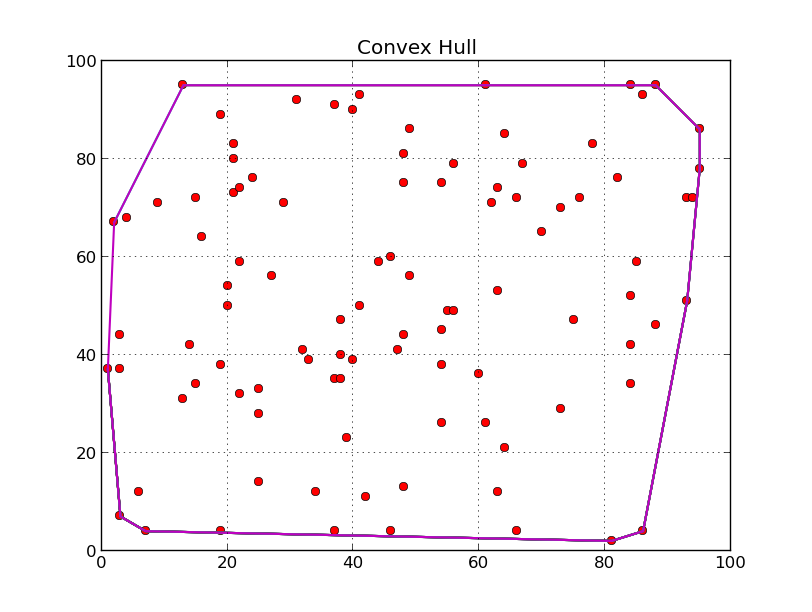
\includegraphics[scale=0.65]{img/monotone_test_1.png}
\end{figure}



\textsc{\large Sample Result 2} \hfill \nspace

\textsc{Input Values} \hfill \nspace

\begin{verbatim}
(4, 3)
(5, 9)
(7, 1)
(2, 7)
(2, 4)
(5, 3)
(5, 7)
(2, 6)
(6, 9)
(3, 2)
\end{verbatim}

% Spacing
\hfill \nspace
\textsc{Points in Hull} \hfill \nspace

\begin{verbatim}
(2, 4)
(3, 2)
(7, 1)
(6, 9)
(5, 9)
(2, 7)
(2, 4)
\end{verbatim}

\newpage
\textsc{Plot} \hfill \nspace

\begin{figure}[h!]
  \centering
	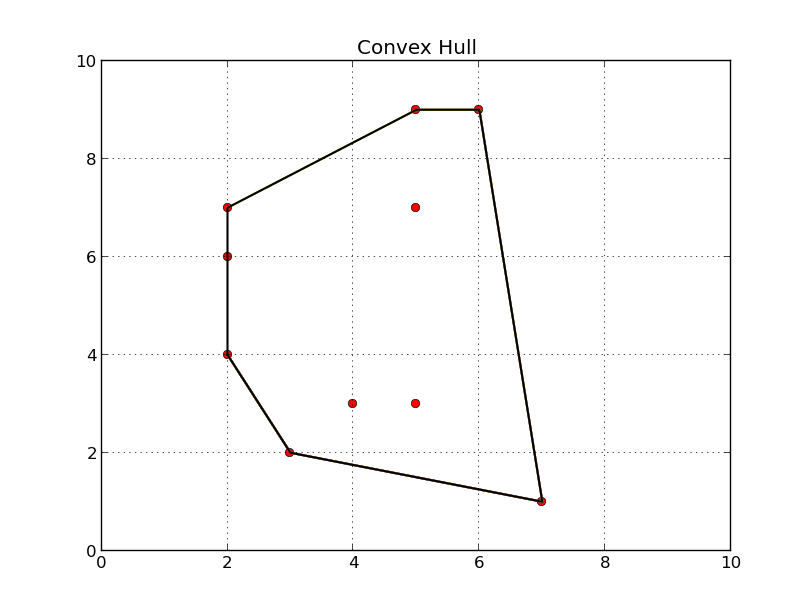
\includegraphics[scale=0.65]{img/monotone_test_2.png}
\end{figure}



\textsc{\large Sample Result 3} \hfill \nspace

\textsc{Input Values} \hfill \nspace

\begin{verbatim}
(4.997518610421837, 8.8775510204081627)
(5.5732009925558312, 8.8520408163265287)
(6.7047146401985103, 8.6734693877551017)
(7.4789081885856081, 8.3418367346938762)
(7.7965260545905704, 7.8571428571428559)
(7.9553349875930515, 7.5765306122448965)
(8.0942928039702231, 7.3979591836734677)
(8.2531017369727042, 6.8877551020408152)
(8.3722084367245646, 6.4285714285714288)
(8.5905707196029777, 5.6887755102040813)
(8.8486352357320097, 4.9489795918367339)
(9.1464019851116625, 3.7499999999999996)
(9.3052109181141436, 3.010204081632653)
(9.2853598014888341, 1.989795918367347)
(8.9677419354838701, 1.3010204081632653)
(8.2332506203473947, 0.58673469387755128)
(7.2009925558312649, 0.2551020408163267)
(6.5062034739454084, 0.20408163265306145)
(5.9305210918114142, 0.12755102040816357)
(5.1960297766749388, 0.2551020408163267)
(4.4019851116625315, 0.45918367346938793)
(3.1910669975186106, 0.91836734693877586)
(3.0322580645161294, 1.0204081632653064)
(2.9131513647642682, 1.1479591836734695)
(2.8337468982630276, 1.25)
(2.694789081885856, 1.4540816326530615)
(2.5161290322580645, 1.7346938775510203)
(2.2779156327543424, 2.0918367346938775)
(2.0397022332506203, 2.5255102040816326)
(1.9801488833746901, 2.8316326530612241)
(1.7022332506203477, 3.7755102040816326)
(1.662531017369727, 4.387755102040817)
(1.7220843672456576, 5.408163265306122)
(1.8014888337468982, 7.3724489795918355)
(1.9007444168734491, 8.0357142857142847)
(2.1191066997518613, 8.3673469387755084)
(2.2580645161290325, 8.5459183673469372)
(2.6550868486352361, 9.0051020408163254)
(2.9131513647642682, 9.1836734693877542)
(3.1315136476426804, 9.2346938775510186)
(3.3895781637717124, 9.2091836734693864)
(3.6277915632754341, 9.1836734693877542)
(3.8660049627791566, 9.1836734693877542)
(4.0248138957816373, 9.1836734693877542)
(4.1439205955334995, 9.1836734693877542)
(4.4019851116625315, 9.1326530612244881)
(4.5210918114143919, 9.1071428571428559)
(4.6600496277915635, 9.0816326530612237)
(4.7990074441687351, 9.0306122448979576)
\end{verbatim}

% Spacing
\textsc{Points in Hull} \hfill \nspace

\begin{verbatim}
(x=1.662531, y=4.387755)
(x=1.702233, y=3.775510)
(x=2.039702, y=2.525510)
(x=2.277916, y=2.091837)
(x=2.694789, y=1.454082)
(x=2.833747, y=1.250000)
(x=2.913151, y=1.147959)
(x=3.032258, y=1.020408)
(x=3.191067, y=0.918367)
(x=4.401985, y=0.459184)
(x=5.196030, y=0.255102)
(x=5.930521, y=0.127551)
(x=7.200993, y=0.255102)
(x=8.233251, y=0.586735)
(x=8.967742, y=1.301020)
(x=9.285360, y=1.989796)
(x=9.305211, y=3.010204)
(x=9.146402, y=3.750000)
(x=8.848635, y=4.948980)
(x=8.253102, y=6.887755)
(x=8.094293, y=7.397959)
(x=7.796526, y=7.857143)
(x=7.478908, y=8.341837)
(x=6.704715, y=8.673469)
(x=4.660050, y=9.081633)
(x=4.143921, y=9.183673)
(x=3.131514, y=9.234694)
(x=2.913151, y=9.183673)
(x=2.655087, y=9.005102)
(x=2.258065, y=8.545918)
(x=2.119107, y=8.367347)
(x=1.900744, y=8.035714)
(x=1.801489, y=7.372449)
(x=1.662531, y=4.387755)
\end{verbatim}



\textsc{Plot} \hfill \nspace

\begin{figure}[h!]
  \centering
	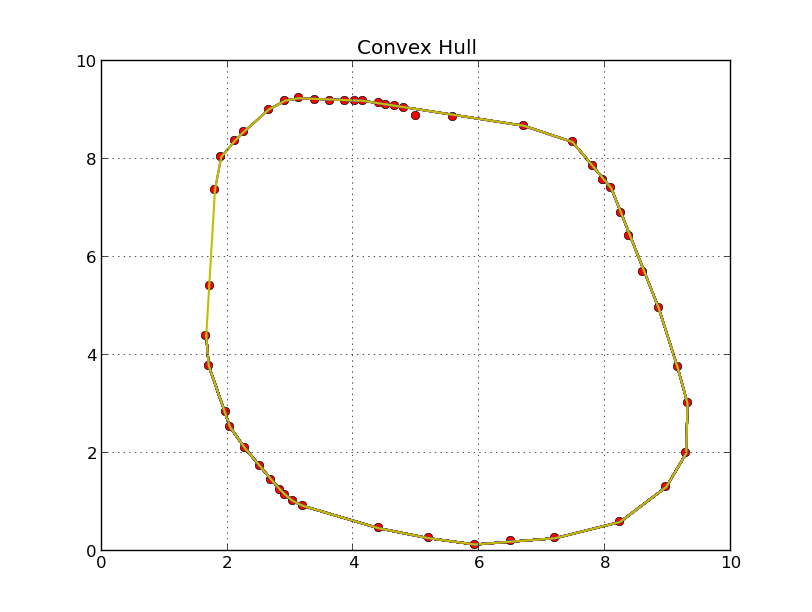
\includegraphics[scale=0.75]{img/monotone_test_3.png}
\end{figure}



\newpage
\textsc{\large Sample Result 4} \hfill \nspace

\textsc{Input Values} \hfill \nspace

\begin{verbatim}
(2.5359801488833749, 8.3928571428571423)
(2.5359801488833749, 8.1632653061224474)
(2.5359801488833749, 7.9591836734693864)
(2.7543424317617871, 7.1173469387755084)
(2.5955334987593051, 6.4795918367346932)
(2.5558312655086852, 5.7908163265306118)
(2.5558312655086852, 4.8214285714285712)
(2.5558312655086852, 4.0561224489795915)
(2.6153846153846154, 3.1887755102040818)
(2.7940446650124069, 3.1377551020408165)
(2.9330024813895785, 3.1122448979591835)
(3.2506203473945408, 3.0612244897959182)
(3.9255583126550868, 3.0867346938775513)
(4.1439205955334995, 3.035714285714286)
(4.7593052109181144, 2.8316326530612241)
(5.1364764267990068, 2.8571428571428572)
(5.5334987593052105, 2.8571428571428572)
(5.7121588089330029, 2.9591836734693877)
(5.8511166253101745, 2.9081632653061225)
(5.9900744416873444, 2.9081632653061225)
(6.0893300248138953, 2.9081632653061225)
(6.2282878411910669, 2.9336734693877546)
(6.3275434243176178, 2.9591836734693877)
(6.5260545905707197, 2.9846938775510208)
(6.6253101736972706, 3.010204081632653)
(6.6848635235732008, 3.0612244897959182)
(6.7047146401985103, 3.3163265306122445)
(6.744416873449131, 3.8775510204081631)
(6.7642679900744405, 4.1326530612244898)
(6.8238213399503724, 5.0510204081632644)
(6.8635235732009914, 5.841836734693878)
(6.9032258064516121, 6.454081632653061)
(6.7642679900744405, 7.1938775510204067)
(6.8436724565756819, 7.7806122448979576)
(6.8833746898263026, 8.112244897959183)
(6.8635235732009914, 8.3418367346938762)
(6.8238213399503724, 8.6989795918367339)
(6.6253101736972706, 8.6479591836734677)
(6.4267990074441688, 8.724489795918366)
(5.9106699751861047, 8.9540816326530592)
(5.2754342431761785, 9.0051020408163254)
(5.1563275434243181, 9.0051020408163254)
(5.0967741935483879, 9.0051020408163254)
(4.7791563275434239, 8.9540816326530592)
(4.6203473945409428, 8.9540816326530592)
(4.4813895781637711, 8.9795918367346932)
(4.3622828784119108, 9.0051020408163254)
(4.2431761786600504, 9.0306122448979576)
(4.0049627791563278, 9.0306122448979576)
(3.885856079404467, 9.0306122448979576)
(3.5880893300248142, 8.9795918367346932)
(2.7741935483870965, 8.8775510204081627)
(2.9925558312655087, 8.9795918367346932)
(3.1513647642679898, 9.0306122448979576)
\end{verbatim}

% Spacing
\hfill \nspace
\textsc{Points in Hull} \hfill \nspace

\begin{verbatim}
(x=2.535980, y=7.959184)
(x=2.555831, y=4.056122)
(x=2.615385, y=3.188776)
(x=2.794045, y=3.137755)
(x=2.933002, y=3.112245)
(x=3.250620, y=3.061224)
(x=4.759305, y=2.831633)
(x=5.533499, y=2.857143)
(x=6.089330, y=2.908163)
(x=6.526055, y=2.984694)
(x=6.625310, y=3.010204)
(x=6.684864, y=3.061224)
(x=6.704715, y=3.316327)
(x=6.764268, y=4.132653)
(x=6.823821, y=5.051020)
(x=6.903226, y=6.454082)
(x=6.883375, y=8.112245)
(x=6.863524, y=8.341837)
(x=6.823821, y=8.698980)
(x=5.910670, y=8.954082)
(x=5.275434, y=9.005102)
(x=4.243176, y=9.030612)
(x=3.151365, y=9.030612)
(x=2.992556, y=8.979592)
(x=2.774194, y=8.877551)
(x=2.535980, y=8.392857)
(x=2.535980, y=7.959184)
\end{verbatim}

\newpage
\textsc{Plot} \hfill \nspace

\begin{figure}[h!]
  \centering
	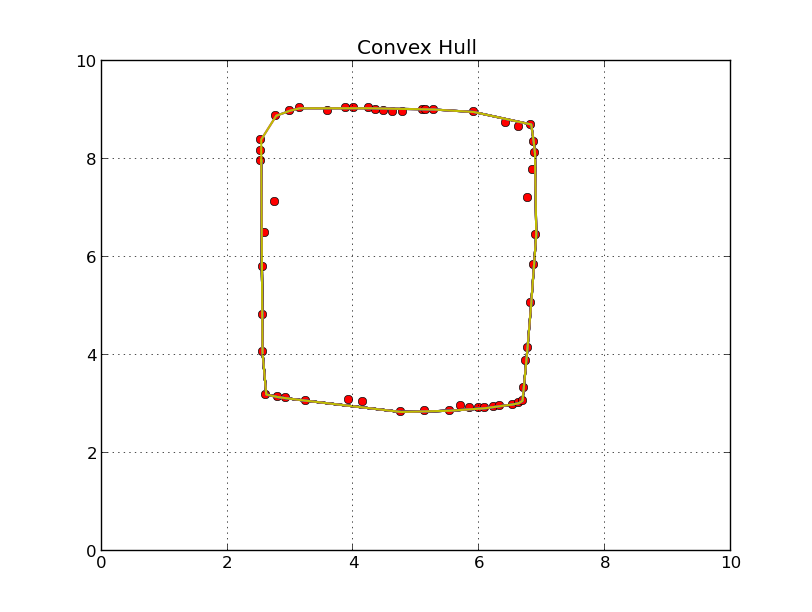
\includegraphics[scale=0.65]{img/monotone_test_4.png}
\end{figure}




% Complexity Analysis
\textsc{\Large Complexity Analysis} \hfill \nspace

{\bf \large 1 Sorting}
\begin{verbatim}
points = sorted(set(points))        nlogn
\end{verbatim}

Sort the points lexicographically using quick sort, first by x-coordinate and when there is a tie, the points will be sorted by y\-coordinate. Since the fastest sort algorthm that can be employeed is of complexity $O(n log n)$ for average and best case, worse case is however $O(n^2)$.\lspace


{\bf \large 2 Single Point Check}
\begin{verbatim}
if len(vectors) <= 1:               1
    return vectors                  1
\end{verbatim}

An initial check is done for if the given list of points is just a single point. Complexity will be $O(1)$.\lspace


{\bf \large 3 Initialize Lower Hull}
\begin{verbatim}
lower = []                          1
\end{verbatim}

Initialize the lower hull's list. The complexity will be O(1).\lspace


{\bf \large 4 Compute Lower Hull}
\begin{verbatim}
for p in vectors:                                                     n
    while len(lower) >= 2 and cross(lower[-2], lower[-1], p) <= 0:    sum(j)
        lower.pop()                                                   sum(j-1)
    lower.append(p)                                                   n                        1
\end{verbatim}

Where \emph{j} is solely based on the given points. \emph{j} will increase if the next point causes a set of the points to be removed as the addition of the next point will cause the previous points to be no longer valid. \emph{j} will decrease if the next point is valid and the previous point is still valid. \emph{j} will always be such that: $j < n$ and such that the summation of $j < n^2$.\nspace

The complexity of finding the lower hull will be such that the summation will be $O(n)$, because:

\begin{equation}
\begin{split}
g(n) &= n + (n + j) + (j-1) + n\\
     &= 3n + 2j - 1\\
     &= O(n)\\
\end{split}
\end{equation}
		
		
{\bf \large 5 Initialize Upper Hull}
\begin{verbatim}
upper = []                        1
\end{verbatim}

Initialize the upper hull's list. The complexity will be will be O(1).\lspace


{\bf \large 6 Compute Upper Hull}
\begin{verbatim}
for p in reversed(vectors):                                           n
    while len(upper) >= 2 and cross(upper[-2], upper[-1], p) <= 0:    sum(j)
        upper.pop()                                                   sum(j-1)
    upper.append(p)
                    1
\end{verbatim}

This is very similar to creating the lower hull except the list is traversed in the opposite direction. The complexity of finding the upper hull will be such that the summation will be 
$O(n)$, because:

\begin{equation}
\begin{split}
g(n) &= n + (n + j) + (j-1) + n\\
     &= 3n + 2j - 1\\
     &= O(n)\\
\end{split}
\end{equation}
		

{\bf \large 7 Merge Hulls}
\begin{verbatim}
return lower[:-1] + upper[:-1]                     1
\end{verbatim}

Once the 2 hulls have been taken they will be merged together. The complexity of the merge will be $O(1)$.\lspace




% Conclusion
\newpage
\textsc{\Large Conclusion} \hfill \nspace

Therefore, given the complexity analysis for each of the operations from 1 to 7 the overall complexity of the Monotone Chain algorithm will be:

\begin{equation}
\begin{split}
f(n) &= O(nlogn) + O(1) + O(1) + O(n) + O(1) + O(n) + O(1)\\
     &= O(nlogn) + O(2n) + O(4)\\
     &= O(nlogn)
\end{split}
\end{equation}
















% Dijkstra's Algorithm
\newpage
\textsc{\Huge Shortest-path Algorithm} \hfill \Lspace

% Description of algorithm (take from wikipedia
\textsc{\Large Description} \hfill \nspace

The shortest path problem is a well-founded problem in graph theory, which involves trying to find the shortest path between two vertices in the graph. In order to facilitate the concept of length in the shortest path problem the graph is weighted such that the shortest path results in the sum of the weights of each edge being the most minimal.\nspace

There are several known algorithms for solving the shortest path problem, such as Dijkstra's Algorithm, Bellman-Ford Algorithm, and A* Search Algorithm.\lspace



% Description of algorithm, explanation of the code
\textsc{\Large Dijkstra's Algorithm} \hfill \nspace

For our project we decided to use Dijkstra's Algorithm, while there are other heuristics-based algorithms which attempt to have better performance. We chose Dijkstra's Algorithm because it still has excellent performance, even in worst case complexity, with $O(|E| + |V| log |V|) $\cite{cormen2001introduction}, where $E$ is the number of edges in the graph, and $V$ is the number of vertices.\nspace

Dijkstra's Algorithm operates by first assigning each vertex a distance value which is used as a weight for the edge. Next, all vertices are marked as unvisited and the initial vertex is marked as current. Then, for each current node calculate the tentative weights or distance of each of it's neighbours that are marked as unvisited, for each distance calculated for the current nodes neighbour, if the distance is less than the previously calculated distance, then overwrite the current distance. Next, when each of the neighbours of the current vertex have been considered mark the current vertex as visited and remove it from the unvisited list. Now, if the destination vertex has been marked as visited then stop, otherwise continue checking the remaining unvisited vertices.\nspace

As part of our research into Dijkstra's Algorithm we looked for detailed explanations of Dijkstra's Algorithm and pseudocode, during our research we found that one of the most detailed and well-explained sources for Dijkstra's Algorithm was from Wikipedia, we used the pseudocode from Wikipedia as a basis for understanding Dijkstra's algorithm and creating our own implementation of Dijkstra's Algorithm in Python.\cite{dijkstrapseudocode}


\begin{footnotesize}
\begin{verbatim}
 1  function Dijkstra(Graph, source):
 2      for each vertex v in Graph:                            // Initializations
 3          dist[v] := infinity ;                              // Unknown distance function from 
 4                                                             // source to v
 5          previous[v] := undefined ;                         // Previous node in optimal path
 6      end for                                                // from source
 7      
 8      dist[source] := 0 ;                                    // Distance from source to source
 9      Q := the set of all nodes in Graph ;                   // All nodes in the graph are
10                                                             // unoptimized - thus are in Q
11      while Q is not empty:                                  // The main loop
12          u := vertex in Q with smallest distance in dist[]; // Start node in first case
13          remove u from Q ;
14          if dist[u] = infinity:
15              break ;                                        // all remaining vertices are
16          end if                                             // inaccessible from source
17          
18          for each neighbor v of u:                          // where v has not yet been 
19                                                             // removed from Q.
20              alt := dist[u] + dist_between(u, v) ;
21              if alt < dist[v]:                              // Relax (u,v,a)
22                  dist[v] := alt ;
23                  previous[v] := u ;
24                  decrease-key v in Q;                       // Reorder v in the Queue
25              end if
26          end for
27      end while
28  return dist;
\end{verbatim}
\end{footnotesize}


% Spacing
\hfill \lspace

% Sample Results
\textsc{\Large Sample Results} \hfill \nspace

\textsc{\large Sample Result 1} \hfill \nspace

\textsc{Input Values} \hfill \nspace

\begin{verbatim}
\end{verbatim}

% Spacing
\hfill \nspace
\textsc{Shortest Path} \hfill \nspace

\begin{verbatim}
\end{verbatim}


\textsc{Plot} \hfill \nspace

\begin{figure}[h!]
  \centering
%	\includegraphics[scale=0.65]{}
\end{figure}


\textsc{\large Sample Result 2} \hfill \nspace

\textsc{Input Values} \hfill \nspace

\begin{verbatim}
\end{verbatim}

% Spacing
\hfill \nspace
\textsc{Shortest Path} \hfill \nspace

\begin{verbatim}
\end{verbatim}


\textsc{Plot} \hfill \nspace

\begin{figure}[h!]
  \centering
%	\includegraphics[scale=0.65]{}
\end{figure}


\textsc{\large Sample Result 3} \hfill \nspace

\textsc{Input Values} \hfill \nspace

\begin{verbatim}
\end{verbatim}

% Spacing
\hfill \nspace
\textsc{Shortest Path} \hfill \nspace

\begin{verbatim}
\end{verbatim}


\textsc{Plot} \hfill \nspace

\begin{figure}[h!]
  \centering
%	\includegraphics[scale=0.65]{}
\end{figure}


\textsc{\large Sample Result 4} \hfill \nspace

\textsc{Input Values} \hfill \nspace

\begin{verbatim}
\end{verbatim}

% Spacing
\hfill \nspace
\textsc{Shortest Path} \hfill \nspace

\begin{verbatim}
\end{verbatim}


\textsc{Plot} \hfill \nspace

\begin{figure}[h!]
  \centering
%	\includegraphics[scale=0.65]{}
\end{figure}

% Complexity Analysis
\textsc{\Large Complexity Analysis} \hfill \nspace

{\bf \large 1 Initialize the dictionaries and arrays}
\begin{verbatim}
D = {}								1
P = {}								1

for node in graph.keys():			n+1
        D[node] = -1				n
        P[node] = ""				n

D[start] = 0						1

unseen_nodes = graph.keys()			1
\end{verbatim}

The distance and the predecessor dictionaries are initialized to unreachable and empty. The start vertex's distance is set to 0 since it is the starting location. The unseen_nodes array is initialized to contain all nodes since every node is unseen.\lspace

{\bf \large 2 Calculate Distances and Predecessors}
\begin{verbatim}
while len(unseen_nodes) > 0:									n+1

    shortest = None												n
    cur_node = ''												n
    for temp_node in unseen_nodes:								sum(j)*
        if shortest == None:									sum(j-1)
            shortest = D[temp_node]								sum(1)**
            cur_node = temp_node								sum(1)
        elif D[temp_node] < shortest:							sum(j-2)
            shortest = D[temp_node]								sum(j-2)
            cur_node = temp_node								sum(j-2)

    unseen_nodes.remove(cur_node)								n

    for child_node, child_value in graph[cur_node].items():		sum(c)`
        if D[child_node] < D[node] + child_value:				sum(c-1)
            D[child_node] = D[node] + child_value				sum(m)~
            P[child_node] = cur_node							sum(m)
\end{verbatim}

This section of the code maps out the distance between the parents and their children. This is done in order from shortest distance to largest, and because if initial conditions the start node is the last node to be checked.
*note that the summations show are from 1 to n
*Also, note that j is the current size of un_seen_nodes which will decrement each iteration
**note that the first if structure is the initial condition therefore it will only enter 1 ever time the for loop takes place
`Please note that c is the number of children that the particular node has. Since this number is completely up to the user the number of iterations can vary greatly. However since a child cannot have it's parent as a child (no recursion) c will be such that c < n and the summation of c < n^2
~Please note that m is the number of times that the condition is successful, since the condition is based on whether the child has already had a parent node pass through it. m is such that it will be m <= c at all times.\lspace

{\bf \large 3 Initialize the path}
\begin{verbatim}
path = []						1
node = end						1
\end{verbatim}

Initialize the path to null and the first node to be checked to the end node.\lspace

{\bf \large 5 Find path to start}
\begin{verbatim}
while not (node == start):					k+1						
    if path.count(node) == 0:				k
        path.insert(0, node)				k-1
        node = P[node]						k-1
    else:									1
        break								1

path.insert(0, start)						1
return path									1
\end{verbatim}

Search for a path to the start node from the end node. Where k is the the number of nodes need to be checked before the start node is found. Given the worse case k will be such k = n therefore k will be k <= n.\lspace

\begin{equation}
\begin{split}
f(n) &= O(1) + O(1) + O(n+1) + O(n) + O(n) + O(1) + O(1) + O(n+1) + O(n) + O(n) + O(j)+  O(j-1) +  O(n) +  O(n) +  O(j-2) + O(j-2) + O(j-2) + O(n) + O(c) + O(c-1) + O(m) + O(m) + O(k+1) + O(k) + O(k-1) + O(k-1) + O(k-1) + O(1) + O(1) + O(1) + O(1) \\
     &= O(14) + O(19n/2) + O(7n^2)\\
     &= O(n^2)
\end{split}
\end{equation}


\bibliographystyle{ieeetr}
\bibliography{references}

\end{document}
